% Options for packages loaded elsewhere
\PassOptionsToPackage{unicode}{hyperref}
\PassOptionsToPackage{hyphens}{url}
%
\documentclass[
]{article}
\usepackage{amsmath,amssymb}
\usepackage{lmodern}
\usepackage{iftex}
\ifPDFTeX
  \usepackage[T1]{fontenc}
  \usepackage[utf8]{inputenc}
  \usepackage{textcomp} % provide euro and other symbols
\else % if luatex or xetex
  \usepackage{unicode-math}
  \defaultfontfeatures{Scale=MatchLowercase}
  \defaultfontfeatures[\rmfamily]{Ligatures=TeX,Scale=1}
\fi
% Use upquote if available, for straight quotes in verbatim environments
\IfFileExists{upquote.sty}{\usepackage{upquote}}{}
\IfFileExists{microtype.sty}{% use microtype if available
  \usepackage[]{microtype}
  \UseMicrotypeSet[protrusion]{basicmath} % disable protrusion for tt fonts
}{}
\makeatletter
\@ifundefined{KOMAClassName}{% if non-KOMA class
  \IfFileExists{parskip.sty}{%
    \usepackage{parskip}
  }{% else
    \setlength{\parindent}{0pt}
    \setlength{\parskip}{6pt plus 2pt minus 1pt}}
}{% if KOMA class
  \KOMAoptions{parskip=half}}
\makeatother
\usepackage{xcolor}
\usepackage[margin=1in]{geometry}
\usepackage{longtable,booktabs,array}
\usepackage{calc} % for calculating minipage widths
% Correct order of tables after \paragraph or \subparagraph
\usepackage{etoolbox}
\makeatletter
\patchcmd\longtable{\par}{\if@noskipsec\mbox{}\fi\par}{}{}
\makeatother
% Allow footnotes in longtable head/foot
\IfFileExists{footnotehyper.sty}{\usepackage{footnotehyper}}{\usepackage{footnote}}
\makesavenoteenv{longtable}
\usepackage{graphicx}
\makeatletter
\def\maxwidth{\ifdim\Gin@nat@width>\linewidth\linewidth\else\Gin@nat@width\fi}
\def\maxheight{\ifdim\Gin@nat@height>\textheight\textheight\else\Gin@nat@height\fi}
\makeatother
% Scale images if necessary, so that they will not overflow the page
% margins by default, and it is still possible to overwrite the defaults
% using explicit options in \includegraphics[width, height, ...]{}
\setkeys{Gin}{width=\maxwidth,height=\maxheight,keepaspectratio}
% Set default figure placement to htbp
\makeatletter
\def\fps@figure{htbp}
\makeatother
\setlength{\emergencystretch}{3em} % prevent overfull lines
\providecommand{\tightlist}{%
  \setlength{\itemsep}{0pt}\setlength{\parskip}{0pt}}
\setcounter{secnumdepth}{-\maxdimen} % remove section numbering
\ifLuaTeX
  \usepackage{selnolig}  % disable illegal ligatures
\fi
\IfFileExists{bookmark.sty}{\usepackage{bookmark}}{\usepackage{hyperref}}
\IfFileExists{xurl.sty}{\usepackage{xurl}}{} % add URL line breaks if available
\urlstyle{same} % disable monospaced font for URLs
\hypersetup{
  pdftitle={Geranium instant report},
  pdfauthor={Boris Solovyev, Nikita Platonov},
  hidelinks,
  pdfcreator={LaTeX via pandoc}}

\title{Geranium instant report}
\author{Boris Solovyev, Nikita Platonov}
\date{2022-12-07 07:57:01}

\begin{document}
\maketitle

\hypertarget{instant-report-for-pac-22.}{%
\subsection{Instant report for PAC 22.}\label{instant-report-for-pac-22.}}

This is dynamically generated report based on passed parameters.

\begin{figure}

{\centering 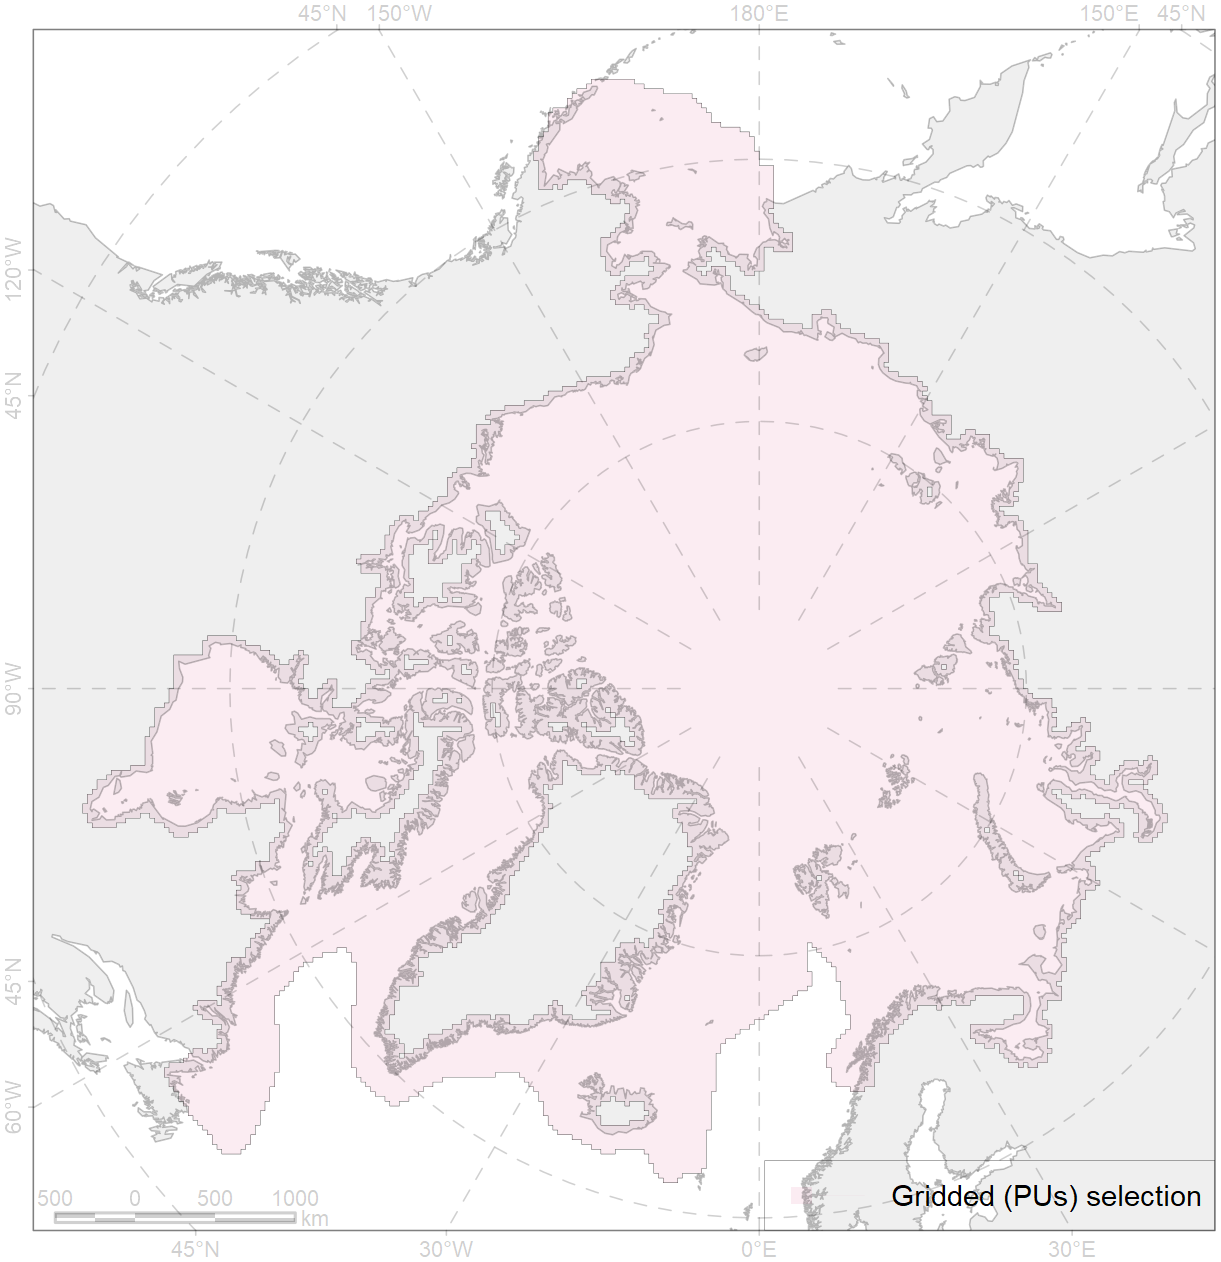
\includegraphics[width=20.12in]{instantReport_files/figure-latex//ursa01_preselectional} 

}

\caption{Selection}\label{fig:selectional}
\end{figure}

The area of selected region is 94580 km\textsuperscript{2}.
This selected area is inscribed into 106 planning units (PUs).
Selected area outside of PUs domain is ignored.
Cellulared (gridded) selection is 95400 km\textsuperscript{2}.
For this gridded selection 81110 km\textsuperscript{2} are aquatories,
and 14290 km\textsuperscript{2} are territories.

There are 43 conservation features (CFs) in selection.
They represent ``Walrus'', ``Pinnipeds'', ``Fishes'', ``Cetaceans'', ``Birds'', ``Benthos'', ``Coastal'', ``Polar bears'' groups of CFs.
Industries represent ``Aquaculture'', ``Fishery'', ``Infrastructure'', ``Mining'', ``Shipping'', ``Tourism'' activity groups.

\begin{table}

\caption{\label{tab:principal}Principal concern indices}
\centering
\begin{tabular}[t]{l|l|r}
\hline
NAO & Conservation concern, not allowed only & 1285.79018\\
\hline
NAC & Conservation concern, not allowed and conditional & 5350.38662\\
\hline
NAOR & Conservation concern, not allowed only relative & 12.13010\\
\hline
NACR & Conservation concern, not allowed and conditional relative & 50.47535\\
\hline
\end{tabular}
\end{table}

\begin{figure}

{\centering 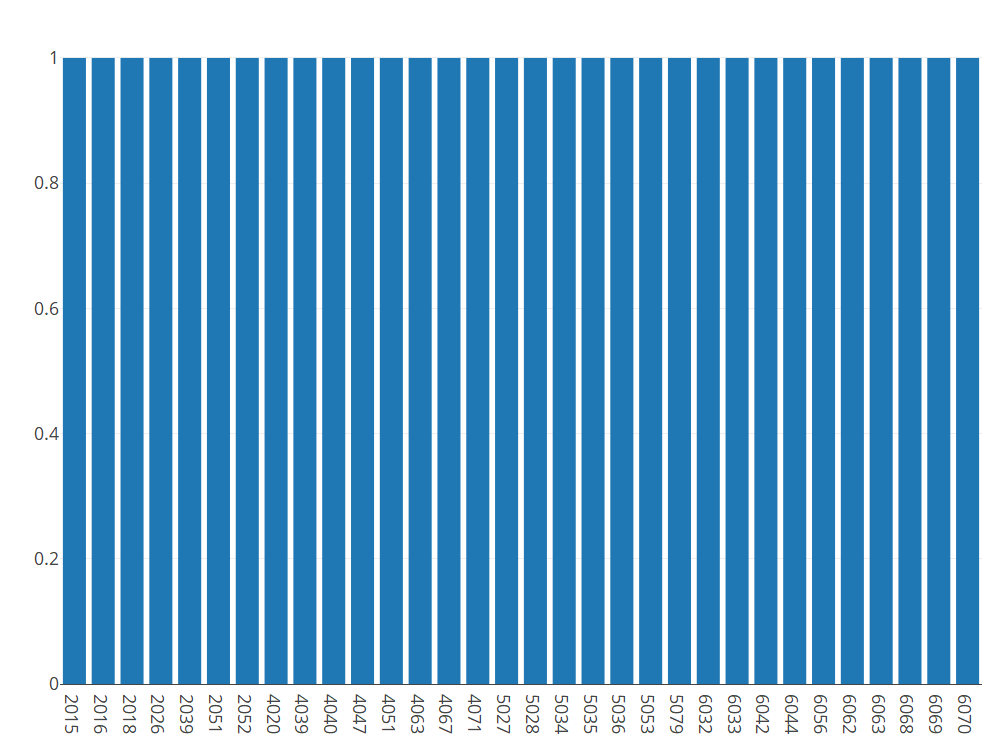
\includegraphics{instantReport_files/figure-latex/residential-1} 

}

\caption{Leading residential CFs in selection}\label{fig:residential}
\end{figure}

\begin{figure}

{\centering 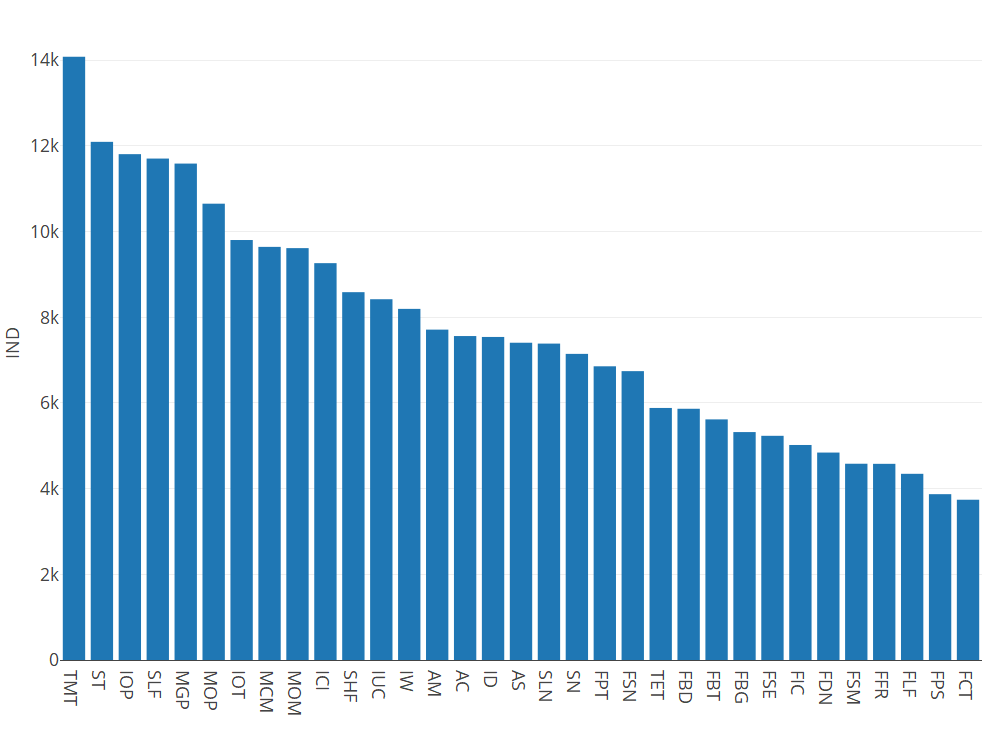
\includegraphics{instantReport_files/figure-latex/industrial-1} 

}

\caption{Industrial concern}\label{fig:industrial}
\end{figure}

\begin{figure}

{\centering 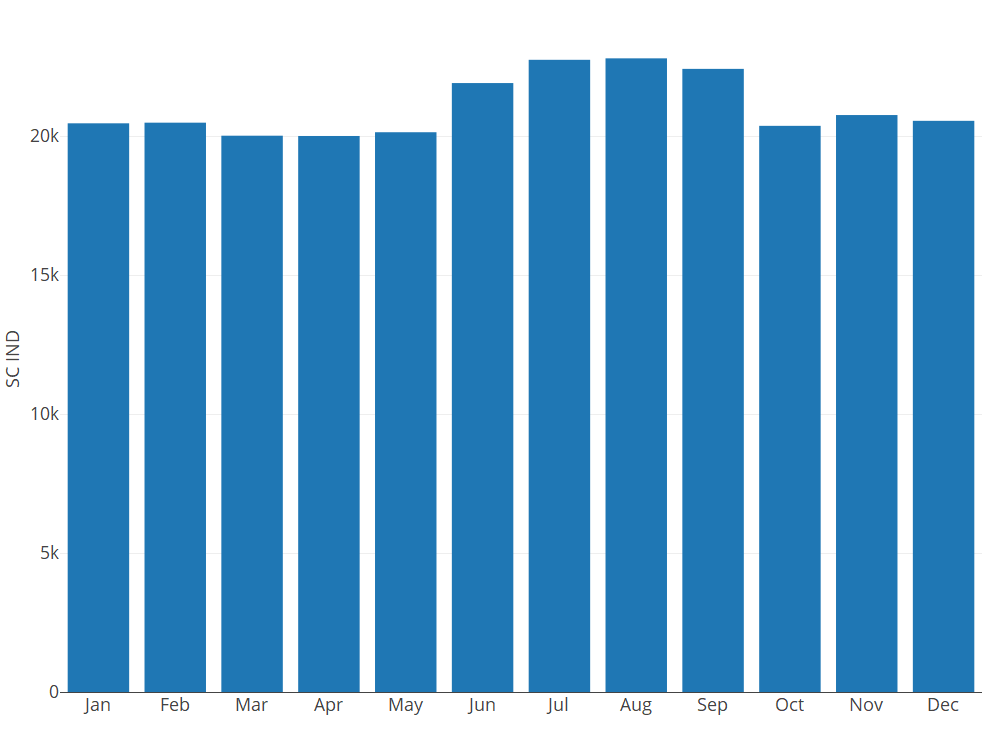
\includegraphics{instantReport_files/figure-latex/seasonal-1} 

}

\caption{Seasonal concern}\label{fig:seasonal}
\end{figure}

\begin{table}

\caption{\label{tab:topind}Industries of concern (TOP IND)}
\centering
\begin{tabular}[t]{l|l|r}
\hline
  & Industry & Concern\\
\hline
SLF & Cargo/Container/Passenger - Light Fuel Oil & 290.5090\\
\hline
ST & Tanker (oil and petrochemicals) & 292.3035\\
\hline
TMT & Mass tourism & 406.1931\\
\hline
\end{tabular}
\end{table}

\begin{table}

\caption{\label{tab:lcind}Industries of least concern (LC IND)}
\centering
\begin{tabular}[t]{l|l|r}
\hline
  & Industry & Concern\\
\hline
FCT & Crab traps & 19.99170\\
\hline
FLF & Longline fishing & 50.20937\\
\hline
FPS & purse seiner & 39.01038\\
\hline
\end{tabular}
\end{table}

\begin{table}

\caption{\label{tab:scind}Seasons of concern (SC)}
\centering
\begin{tabular}[t]{l|r}
\hline
  & Concern\\
\hline
Jun & 516.5389\\
\hline
Jul & 514.1207\\
\hline
Aug & 514.5262\\
\hline
\end{tabular}
\end{table}

\end{document}
